\documentclass[journal]{IEEEtran}
\usepackage{xcolor}
\usepackage{cite}
\usepackage{amsmath,amssymb,amsfonts}
\usepackage{algorithm}
\usepackage{algpseudocode}
%\usepackage{algorithmic}
\usepackage{graphicx}
\usepackage{textcomp}
\usepackage{graphicx}
%\usepackage{caption}
\usepackage{subcaption}
\usepackage[hyphens]{url}

% correct bad hyphenation here
% \hyphenation{op-tical net-works semi-conduc-tor}

\begin{document}

\title{ELEC1601 Exercise * Lab Report}

\author{SID: ********, Lab Group: *****}

% make the title area
\maketitle


\begin{abstract}
Very briefly: What was the goal of this work? What you did you do to achieve this? What did you learn?
\end{abstract}


\section{Introduction}

\IEEEPARstart{T}{he} purpose of this lab session was … (what you think we want you to learn/skills we want you to develop)

Overview the methods that you used to achieve the learning outcomes you just stated, including software, hardware and teamwork.

State what  you achieved in your final implementation.

\section{Background}
Overview any related background information. This should include components and tools used in lab (include all components: LEDs, resistors, diodes). For every component that is not minor (e.g. wires), you should discuss briefly what they do/how they work (E.g. under what conditions does an LED produce light, what affects it’s brightness), how you will use them. Furthermore, give examples of real-world uses of these components (e.g. LEDs are increasingly used in lighting rooms, but also indicators for digital devices.

You can, but do not have to use the following sub-headings:

\subsection{Tools (e.g TinkerCAD/ Arduino IDE)}
\subsection{Computer (Arduino)}
\subsection{Sensors (outputs)}
\subsection{Actuators (outputs)}
\subsection{Other materials (wires/resistors)}

You can, but do not have to use tables. If you do, an example of how you might format one is given in Table ~\ref{tab1}, which describes a summary of all the materials required for this laboratory exercise.

\newpage
\begin{table}[htbp]
\caption{Summary of all components. (You can, but do not have to include this table. This table example is an example of how to add a table to  your document, and how to construct in Latex)}
\begin{center}
\begin{tabular}{|c|c|c|}
\hline
\textbf{Component} & \textbf{\textit{Number required}}& \textbf{\textit{Other details}}\\
\hline
LED& 4 &  \\
Resistor& 10 &  330 Ohm\\
\hline
\end{tabular}
\label{tab1}
\end{center}
\end{table}

\section{Method}
For each part of the lab, describe the circuit you created, and describe your code with pseudocode. Explain what this pseudocode does and how it interacts with your circuit drawing using text in this section. Explain any design decisions made (why use LED/how you chose your values to send from Arduino to the LED, why you chose a given resistor size if important). Discuss any limitations/successes/unexpected results.

Highlight how you built on aspects you created in earlier parts of the lab where possible).

Describe any differences/challenges in moving from software to hardware..

Use Figures/Tables/Algorithms as appropriate.

\subsection{Part I}
(Example text of how to cite/how to reference tables). In Part 1, we emulated the circuit described in the lab instructions \cite{elec1601_notes} (this is how we write a reference). Another example is the book by Harris and Harris~\cite{harris2010digital}. Algorithm~\ref{alg:part1} (Example how to reference an algorithm). Describes our program to make this circuit run. (Please note, pseudocode is code that describes the algorithm in such a fashion it can be easily translated into any programming language. It should not have any specific syntax e.g. C/JAVA/Python)


\begin{algorithm}
\caption{Psuedocode for Part 1 (please note, this is not correct, just giving you an idea of what pseudo code should look like}\label{alg:part1}
\begin{algorithmic}[1]
\State Assign button to an input pin
\State Assign LED to an output pin
\State READ button input pin
\If{button pressed} 
    \State Make LED output pin high
\Else
    \State Make LED output pin low
\EndIf 
\end{algorithmic}
\end{algorithm}

\subsection{Part II}
\subsection{Part III}
\subsection{Part IV}
(Example text of how to use subfigures). For this part, we were not provided a circuit diagram or design. Figure~\ref{fig:Circuit_diagram} shows our circuit diagram and Figure~\ref{fig:connections} shows a representation of how the components can be wired up to the Arduino.

\begin{figure}[ht]
    \centering
      \begin{subfigure}[b]{0.2\textwidth}
         \centering
         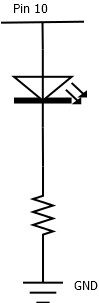
\includegraphics[width=0.3\textwidth]{images/LED.png} 
         \caption{Circuit Diagram}
         \label{fig:Circuit_diagram}
     \end{subfigure}
     \begin{subfigure}[b]{0.2\textwidth}
         \centering
         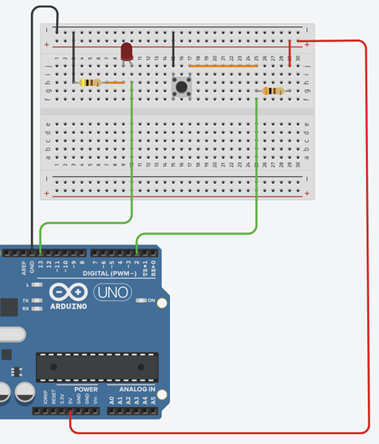
\includegraphics[width=0.9\textwidth]{images/lab_report_pic.png} 
         \caption{Diagram of connections}
         \label{fig:connections}
     \end{subfigure}  \hfill
    \caption{Circuit diagram and connection representation of Part IV (please note, these are obviously not related. This is an example of how to create a figure)}
    \label{fig:part1}
\end{figure}

\section{Results}
Describe the success/failure of your work.
Highlight any limitations! (this shows understanding)

\section{Relation to real-world electronics}

Describe how what you learnt in this lab exists as part of a real devices/products you use, or as an alternative, describe a project you could invent based on what you have learnt.
For this section, you can move beyond an Arduino, but it should be based on  sensors/actuators related to the lab exercise.

Example: a light sensor could be connected to alarm to remind you to put on sunscreen. However, try to elaborate here (e.g. it connects via wifi to your phone and creates a notification). 

\begin{itemize}
  \item Discuss connections/sensors (suggest what is required to implement this - use drawings as necessary).
  \item Discuss pseudo code required to get it to work (this can be very high level (e.g. detect light level -> test against threshold -> send information via wifi to phone) 
  \item Discuss challenges, risks and difficulties to get it working/what could go wrong (e.g calibration for different environments)/fragility of components. Also discuss safety issues.
\end{itemize}

\section{Conclusion}
Describe to what extent your stated learning outcomes were met and what you learnt.

\bibliographystyle{ieeetr}
\bibliography{references/ref}

\appendix

Any additional information. Please be aware, anything in this section may not be marked - it cannot contain anything critical. 

\end{document}

